Les diagrammes de classes participantes sont représentés dans cette 
partie. Il y en a un par cas d'utilisation.

\section{Se connecter au bureau distribué}

\noindent\begin{figure}[H]
	\centering
	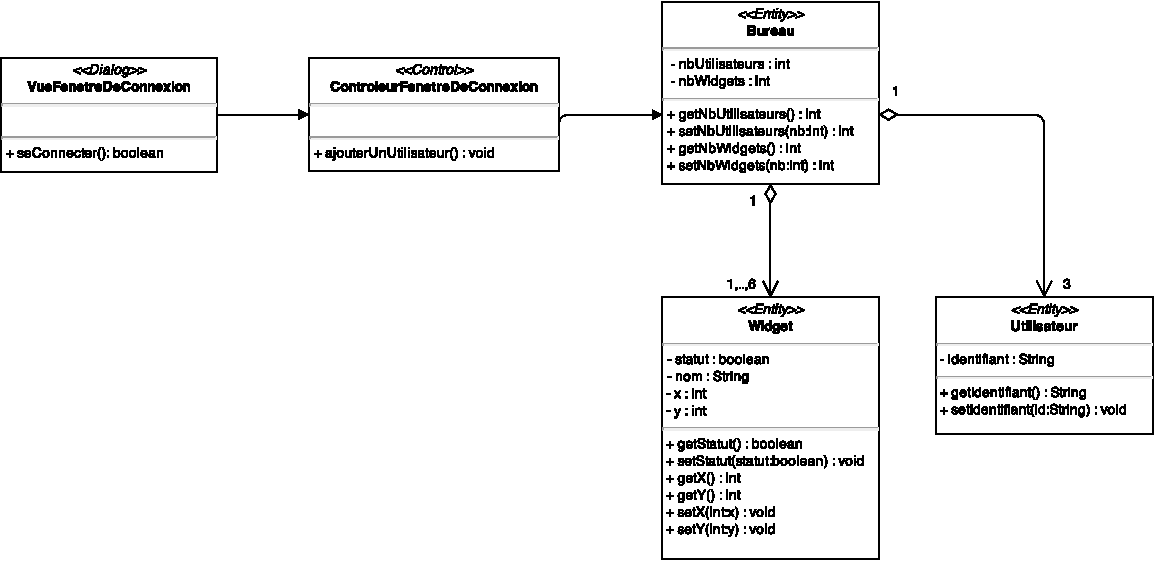
\includegraphics[angle=90,scale=0.8]{diagrammes/DCP1.pdf}
	\caption{Diagramme de Classes Participantes, cas 1}
\end{figure}

\section{Ouvrir une fenêtre}

\begin{figure}[H]
	\centering
	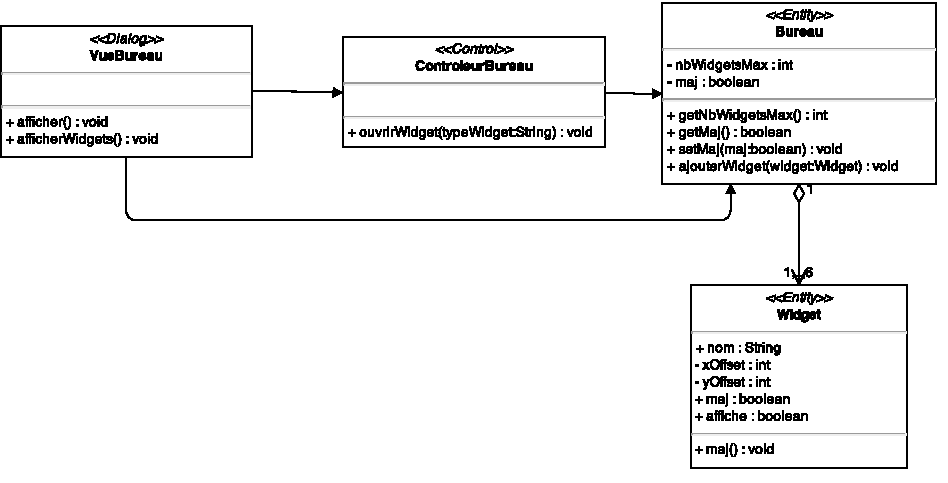
\includegraphics[angle=90]{diagrammes/DCP2.pdf}
	\caption{Diagramme de Classes Participantes, cas 2}
\end{figure}

%\section{Fermer un widget}
%\begin{figure}[H]
%	\centering
%	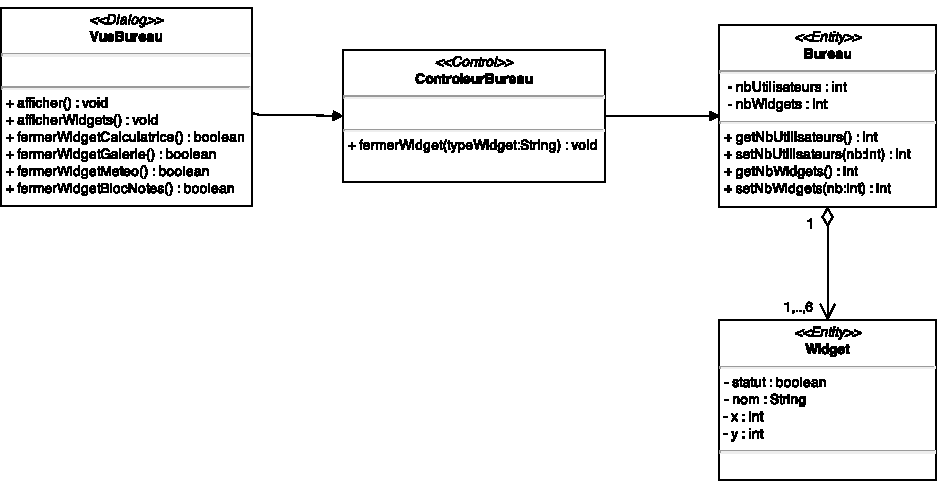
\includegraphics[angle=90]{diagrammes/DCP3.pdf}
%	\caption{Diagramme de Classes Participantes, cas 3}
%\end{figure}

\section{Saisir une opération}
\noindent\begin{figure}[H]
	\centering
	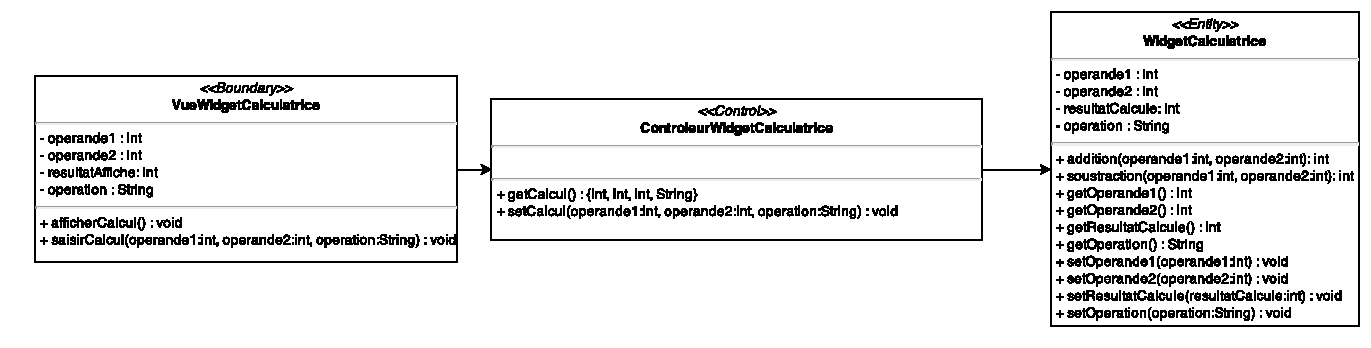
\includegraphics[angle=90,scale=0.9]{diagrammes/DCP4.pdf}
	\caption{Diagramme de Classes Participantes, cas 4}
\end{figure}

\section{Regarder des photos}
\begin{figure}[H]
	\centering
	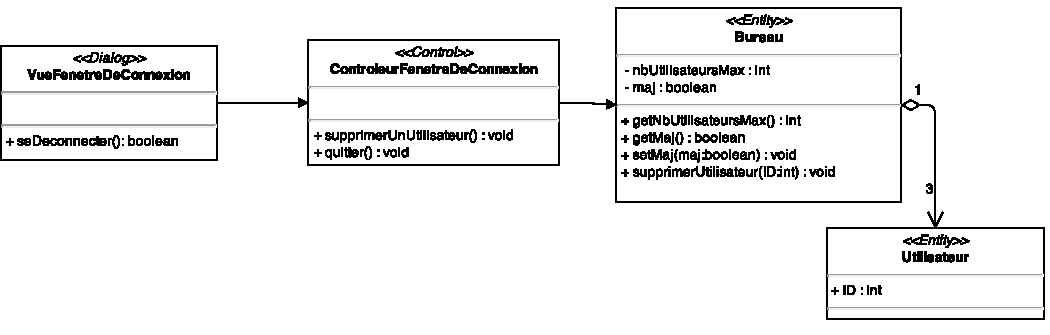
\includegraphics[angle=90]{diagrammes/DCP5.pdf}
	\caption{Diagramme de Classes Participantes, cas 5}
\end{figure}

\section{Quitter le bureau virtuel}

\begin{figure}[H]
	\centering
	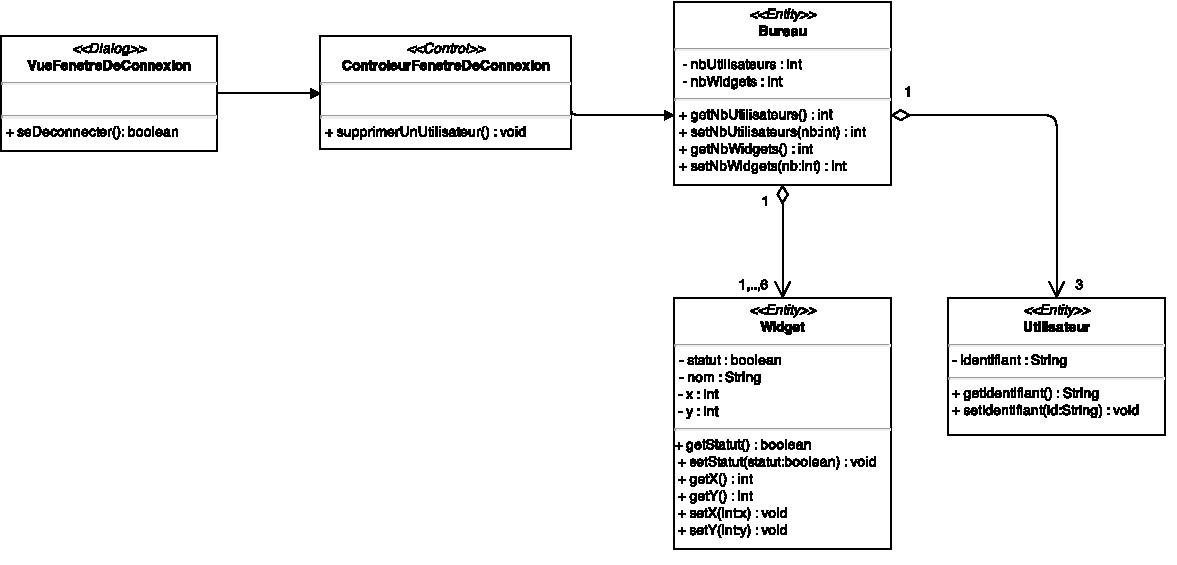
\includegraphics[angle=90]{diagrammes/DCP6.pdf}
	\caption{Diagramme de Classes Participantes, cas 6}
\end{figure}